\documentclass[a4paper,oneside,12pt]{report}


\usepackage[utf8]{inputenc}
\usepackage[T1]{fontenc}
\usepackage[ngerman]{babel}
\usepackage{graphicx}
\usepackage{setspace}

\graphicspath{ {./Images/} }
\usepackage{listings}
\lstset{
	inputpath={./Code/},
	language=Python,
	basicstyle=\tiny,
	numbers=left,
	stepnumber=1,
	showstringspaces=false,
	tabsize=1,
	breaklines=true,
	breakatwhitespace=false,
}


\usepackage{gensymb}

\usepackage{chngcntr}
\counterwithout{footnote}{chapter}
\counterwithout{figure}{chapter}
\counterwithout{table}{chapter}

%Adjust the page margins 
\usepackage[left=3cm, right=3cm, top=2cm, bottom=2cm, a4paper, portrait]{geometry}

%For fancy headers and footers
\usepackage{fancyhdr}
\usepackage{mathpazo}
%Change captions
\usepackage[font=footnotesize,labelfont=bf,tableposition=top]{caption}
%Enable link support in the pdf
\usepackage{hyperref}
%Using BibLaTeX (replacing BibTeX)
\usepackage[autostyle,german=guillemets]{csquotes}
\usepackage[natbib=false,citestyle=numeric-comp,bibstyle=numeric-comp,sortcites=true,backend=biber]{biblatex}
\bibliography{template_advanced_thesis_references}


%Adjust headings and footers --> \usepackage{fancyhdr}
%Give the headings some space
\setlength{\headheight}{15pt}
%This is valid for all pages exept chapters
\pagestyle{fancy}
\fancyhf{} % clear all headers and footers
\rhead[\thepage]{{\leftmark}}
\rfoot[{\leftmark}]{\thepage}
\renewcommand{\headrulewidth}{0.4pt}
% For \chapters \maketitle
\fancypagestyle{plain}{%
	\fancyhf{} % clear all header and footer fields
	\rfoot[{\leftmark}]{\thepage}%
	\renewcommand{\headrulewidth}{0pt}
	\renewcommand{\footrulewidth}{0pt}
}




%Adjust hyperlink behavior -> \usepackage{hyperref}
\hypersetup{
	%bookmarks=true,        										 % show bookmarks bar?
	unicode=false,         											 % non-Latin characters in Acrobatics bookmarks
	pdftoolbar=true,      											 % show Acrobatics toolbar?
	pdfmenubar=true,       											 % show Acrobatics menu?
	pdffitwindow=false,     										 % window fit to page when opened
	pdfstartview={FitH},   											 % fits the width of the page to the window
	pdftitle={FWP Grundlagen der kuenstlichen Intelligenz},    		 % title
	pdfauthor={Maximilian Anzinger, Michael Mican, Philipp Muhr} 	 % author
	pdfsubject={Ampelphasenerkennung},    							 % subject of the document
	pdfkeywords={Kuenstliche Intelligenz, Informatik}, 				 % list of keywords
	pdfnewwindow=true,     											 % links in new window
	colorlinks=true,        										 % false: boxed links; true: colored links
	linkcolor=black,       											 % color of internal links
	citecolor=black,      											 % color of links to bibliography
	filecolor=black,      											 % color of file links
	urlcolor=black        											 % color of external links
}


%Absatzzeilen verhindern
\clubpenalty = 10000
\widowpenalty = 10000 
\displaywidowpenalty = 10000




\begin{document}

	\pagenumbering{alph}  % numbering a, b, c
	\pagenumbering{arabic} % numbering arabic
	
\begin{titlepage}
	\begin{center}
		
		\textsc{\scshape \huge Prüfungsstudienarbeit (PStA)}\\
		\rule{1\textwidth}{1mm} \\[0.5cm]
		{ \LARGE  {\bfseries Technische Hochschule Deggendorf}}\\[0.5cm]
		{ \LARGE   Fakultät Elektrotechnik, Medientechnik und Informatik}\\[0.5cm]
		\rule{1\textwidth}{1mm} \\[4cm] 
		{ \Large \bfseries Thema: Ampelphasenerkennung}\\[2cm]
		{ Fach: FWP Grundlagen der künstlichen Intelligenz}\\[5cm]
		
		\begin{minipage}{0.4\textwidth}
			\begin{flushleft} \normalsize
				\emph{vorgelegt von:}\\[0.3cm]
				Philipp Muhr, Michael Mican, Maximilian Anzinger\\[0.2cm]
				Deggendorf,  \today
			\end{flushleft}
		\end{minipage}
		\begin{minipage}{0.5\textwidth}
			\begin{flushright} \normalsize
				\emph{Prüfer:}\\[0.3cm]
				Prof. Dr. Andreas \textsc{Fischer}\\[0.2cm]
			\end{flushright}
		\end{minipage}\\[2cm]
		{\large \today}
				
	\end{center}
\end{titlepage}

	
	%Inhaltsverzeichnis
	\tableofcontents
	\cleardoublepage
	
	
	\chapter{Einleitung}
	%Link zu den Kapiteln inkl. Inhaltsverzeichnis
	\begin{onehalfspace}
		Im Straßenverkehr finden sich viele Herausforderungen. Es müssen viele Situationen vorausgesehen werden, um eine sichere Fahrt zu gewährleisten. Bei immer höher werdenden Verkehrsaufkommen werden es die Fahrer auch in Zukunft nicht einfach haben. Damit die Verkehrssituation sicherer gestaltet werden kann, werden Unmengen an verschiedenen Fahrassistenzsystemen entwickelt. Diese Studienarbeit behandelt ein Assistenzsystem zur leichteren Ampelphasenwahrnehmung. Eine rote Ampel wird schnell übersehen, daher muss auch in dieser Thematik unterstützte Wahrnehmung begünstigt werden. Es soll ein neuronales Netz trainiert werden, das Ampeln und deren unterschiedlichen Schaltphasen (rot, rot-gelb, gelb und grün) erkennen kann. Ziel dieser künstlichen Intelligenz soll sein, dass sie den Fahrer durch Statusmeldungen in beispielsweise dem Bordmonitor mit der aktuellen Ampelphase informiert. Falls die Sicht des Mobilisten eingeschränkt ist und dieser die Phasen der Ampel nur schwer bis gar nicht erkennen kann, soll er sich auf die Anzeige der Ampelerkennung im Bordmonitor verlassen können. Diese Arbeit wird Aufschluss geben, wie die künstliche Intelligenz aufgebaut und trainiert wurde. Außerdem werden unterschiedliche Verfahren im Bereich Image processing beschrieben, um eventuell performantere Ergebnisse zu erzielen. Im ersten Kapitel wird dargelegt, auf welchem neuronalen Netz aufgebaut wurde und wie dieses angelegt wurde.
	\end{onehalfspace}

	\chapter{Netzwerk}
	\begin{onehalfspace}
		Wie bereits erwähnt soll die Erkennung der Ampel beziehungsweise weiterführend die Phase dieser durch ein neuronales Netz realisiert werden.\\
		Mittlerweile gibt es viele verschiedene Neuronale Netze zur Erkennung von Objekten in Bildern und/oder Videos (Object Recognition). Als Basis dient hier meist ein sogenanntes Convolutional Neural Network (CNN), welches aus mehreren namensgebenden Convolutional Layern, Pooling Layern, einem Fully Connected Layer sowie einer Softmax Funktion besteht.
		Dieses Konzept wird dann um verschiedene Operatoren, Funktionen oder Ähnliches erweitert.\\
		Im Nachfolgenden wird das, von uns genutzte, Netzwerk YoloV3-tiny genauer erklärt beziehungsweise allgemein auf das Konzept von YOLO eingegangen.
		\section{YOLO}
		\subsection{Yolo allgemein}
		YOLO ist laut offizieller Aussage ein "`Echtzeit Objekterkennungs System"'
		\footnote{"https://pjreddie.com/darknet/yolo/", besucht am 30.05.2020 (eigene Übersetzung)},
		welches vorallem auf Geschwindigkeit bei gut bleibender Genauigkeit setzt.\\
		Es nutzt im Gegensatz zu vielen herkömmlichen Objekterkennungsnetzen, wie beispielsweise Faster-RCNN oder Mask-RCNN, nicht mehrere Netze hintereinander, sondern lediglich ein Einziges. Bei den eben genannten Netzwerken wird als erstes ein sogenanntes Region Proposal Network genutzt (welches relevante Regionen herausfiltert). YOLO hingegen geht "`einen völlig anderen Weg und schaut nur ein einziges Mal auf das Bild"
		\footnote{"https://www.sigs-datacom.de/trendletter/2018-10/4-wie-man-in-echtzeit-mehrere-objekte-mit-deep-learning-und-yolo-erkennen-und-klassifizieren-kann.html", besucht am 30.05.2020}
		und "`erkennt gleichzeitig alle interessanten Bereiche und klassifiziert diese mit eine[m] Score."
		\footnote{"https://www.sigs-datacom.de/trendletter/2018-10/4-wie-man-in-echtzeit-mehrere-objekte-mit-deep-learning-und-yolo-erkennen-und-klassifizieren-kann.html", besucht am 30.05.2020}\\
		Diese Technik ermöglicht es, dem Netzwerk eine deutlich schnellere Klassifizierung vorzunehmen. 
		Jedoch bringt diese Geschwindigkeit, beziehungsweise diese Technik auch einen Nachteil mit sich. Für ein solches Modell ist es schwieriger ein sehr kleines Objekt zu erkennen, da das Grid, welches auf das Bild gelegt wird sehr "grob"\space im Vergleich zu anderen Netzen ist. \\
		Deshalb ist ein Modell, wie zum Beispiel Retinanet mit einem Backbone wie einem FPN (Feature Pyramid Network) deutlich besser in der Erkennung von kleinen Objekten bzw. auch in der Genauigkeit der Vorhersagen generell, auch wenn dies natürlich Performance kostet. (vgl. Abbildung~\ref{fig:comparison}
		\footnote{"https://syncedreview.com/2018/03/27/the-yolov3-object-detection-network-is-fast/", besucht am 30.05.2020})\\
		\begin{figure}[h!]
			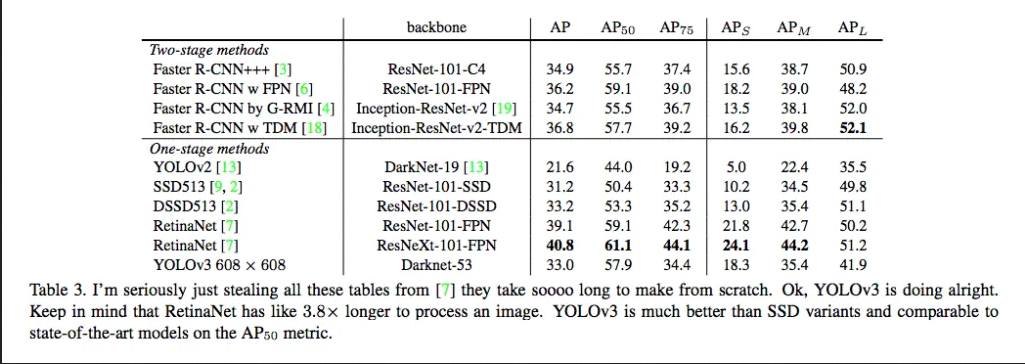
\includegraphics[width=\linewidth]{Comparison.png}
			\caption{Yolov3 Comparison}
			\label{fig:comparison}
		\end{figure}
		\subsection{YoloV3-tiny}
		Für unseren Einsatzfall lohnt es sich, wie oben beschrieben, einen Blick auf Tiny Yolo zu werfen. \\
		Ein "`ganzes"\space YOLO Netzwerk, wie zum Beispiel das neue YoloV4 oder das gängige YoloV3 Modell, bieten gute Ergebnisse, jedoch ist die Performance dieser auf einem Nvidia Jetson Nano Gerät leider zu schlecht, um diese dem Nutzer direkt "`live"\space weitergeben zu können.
		Daher wird eine "`kleine"\space Version von Yolo (genannt Tiny-Yolo) für diesen Anwendungsfall genutzt. Tiny-Yolo (V3) kann Bilder auf einem Nvidia Jetson Nano mit ca. 25 Bildern pro Sekunde klassifzieren und bietet somit eine, für diese Platform, sehr gute Performance.\clearpage
		Aufgrund dieser deutlich höheren Performance (ca. 6,2x die Geschwindigkeit von YoloV3-416) verschlechtert sich die Genauigkeit jedoch auch um ca. 40\% (vgl. Abbildung~\ref{fig:yolov3-tiny}) \\
		Im Hinblick auf die begrenzte Rechenleistung von Mikrocontrollern wird unser Modell mit Tiny-Yolo realisiert, um das Netzwerk auf einem solchen Gerät lauffähig zu machen.
		\begin{figure}[h!]
			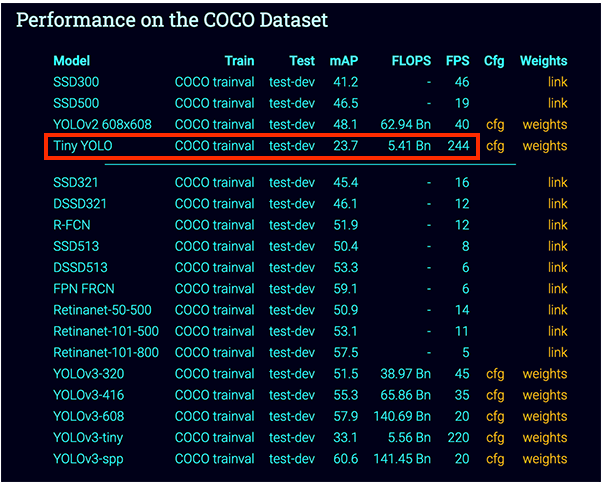
\includegraphics[scale=0.7]{YoloV3-tiny.png}
			\caption{Yolov3(-tiny) Comparison}
			\label{fig:yolov3-tiny}
		\end{figure}
	\end{onehalfspace}
	\chapter{Realisierung}
	\begin{onehalfspace}
		Wie schon in der vorherigen Sektion erwähnt, soll das Projekt auf einem Nvidia Jetson Nano realisiert werden. Dieser bietet für seinen vergleichsweise niedrigen Preis (ca. 99\$
		\footnote{"https://nvidianews.nvidia.com/news/nvidia-announces-jetson-nano-99-tiny-yet-mighty-nvidia-cuda-x-ai-computer-that-runs-all-ai-models", besucht am 31.05.2020})
		im Hinblick auf Inferenz eine sehr gute Performance für die Kosten.
		\section{Hardware}
		Der Nvidia Jetson Nano berechnet mit seiner 128 Kern Nvidia Maxwell Grafikeinheit und seinem Quad-Core ARM Cortex -A57 laut Nvidia 472 GFLOPs.
		\footnote{"https://developer.nvidia.com/embedded/develop/hardware", besucht am 31.0.5.2020}
		Das Gerät wird für unseren Anwendungsfall zusätzlich mit einer Raspberry Pi Camera v2.1 ausgestattet, welche den Videostream liefert. Das Nvidia System ermöglicht eine Video Dekodierung von bis zu vier gleichzeitigen Full-HD Streams bei 30 Bildern pro Sekunde bzw. analog von acht bei 30 Bildern pro Sekunde.
		\footnote{"https://developer.nvidia.com/embedded/develop/hardware", besucht am 31.0.5.2020}
		\section{Software}
		Nvidia schafft es, bei der Jetson Platform die Geräte sehr gut zu optimieren beziehungsweise die Hardware optimal zu nutzen. Dies ermöglichen Frameworks, wie beispielsweise Deepstream und/oder TensorRT
		\subsection{Deepstream}
		Deepstream ist ein Software Development Kit, das "`ein beschleunigtes AI Framework darstellt, welches zur Erstellung von Intelligenten Video Analyse Pipelines genutzt wird."
		\footnote{"https://docs.nvidia.com/metropolis/deepstream/dev-guide/", besucht am 31.05.2020 (eigene Übersetzung)}
		Deepstream fungiert als "`Schnittstelle"\space zwischen Python, C, C++ Applikationen und der Platform selbst (zum Beispiel einem Nvidia Jetson Nano / TX2).
		Weiterführend basiert es auf CUDA (einer GPU basierten parallelen Programmiersprache, die meist bei neuronalen Netzen zum Einsatz kommt), welches TensorRT nutzt.
		\subsection{TensorRT}
		TensorRT ist, analog zu Deepstream, auch ein Software Development Kit, welches für "high-performance deep learning inference"
		\footnote{"https://developer.nvidia.com/tensorrt", besucht am 31.05.2020} genutzt werden kann.
		Applikationen, die auf TensorRT basieren, können bis zu 40 mal schneller sein als vergleichbare Applikation, die auf einer CPU berechnet werden.
		\footnote{"https://developer.nvidia.com/tensorrt", besucht am 31.05.2020}
		Dieses SDK konvertiert ein trainiertes neuronales Netzwerk mithilfe eines TensorRT Optimizers in eine TensorRT Runtime Engine. Dies geschieht durch die Kombinierung von Layern und Optimierung der Kernel-Auswahl.
		\footnote{"https://docs.nvidia.com/deeplearning/tensorrt/developer-guide/index.html", besucht am 31.05.2020}
		Durch diese Umwandlung beziehungsweise Optimierung des Netzwerkes, kann ein enormer Geschwindigkeitsgewinn, wie oben beschrieben, erzielt werden. \\
		Im nächsten Kapitel wird das manuelle Klassifizieren verschiedener Bilder genauer erläutert.
	\end{onehalfspace}
	\chapter{Labeling}
	\begin{onehalfspace}
		 Labeln ist der Vorgang, bei dem in unterschiedlichen Bildern Objekte markiert werden, die die künstliche Intelligenz später als definierte Klasse identifizieren soll. Dieses Kapitel beschreibt, wie beim Labeln vorgegangen wurde. Dabei wird zunächst auf die Datenbeschaffung eingegangen.
		\section{Datenbeschaffung / Open Image Dataset (OID)}
		Anfangs wurden durch das OIDv4\_ToolKit\footnote{"https://github.com/TheAiGuysCode/OIDv4\_toolkit", besucht am 01.06.2020} 
		Bilder aus dem Open Image Dataset (OID) von Google heruntergeladen. Die Bilder waren bereits nach Thematik Ampel beziehungsweise Straßenschilder gelabelt. Leider konnte der Datensatz so nicht direkt verwendet werden, da unsere künstliche Intelligenz auch die Ampelphasen erkennen soll. Ergo wurden alle Bilder mithilfe von Yolo\_Label\footnote{"https://github.com/developer0hye/Yolo\_Label", besucht am 01.06.2020} 
		neu klassifiziert. Was außerdem erwähnt werden muss, ist die Unterstützung familiärer Seite, welche bei der Beschaffung von Bildern der Ampelphasen und Straßenschildern nachgeholfen haben, indem Bilder selbst aufgenommen wurden. Das half vor allem der Erkennung von rot-gelb und gelb Phasen bei Ampeln, da wenige Aufnahmen dieser Phasen im OID vorhanden waren. Da diese Bilder nicht nach den nötigen Anforderungen gelabelt waren, wurden diese mithilfe von Yolo\_Label manuell klassifiziert. Dieses Tool wird im nächsten Abschnitt beschrieben.
		\section{Yolo\_Label}
		Yolo\_Label ist ein Bearbeitungstool, mit dem Objekte in einem Bild durch einen rechteckigen Rahmen, beispielsweise zum Trainieren einer künstliche Intelligenz, gekennzeichnet werden können. Dazu wird ein Datensatz mit einer Menge an Bildern für die entsprechende Thematik benötigt. Weiterhin muss eine Textdatei erstellt werden, in der die gewünschten Klassen, wie zum Beispiel "`rote Ampel"' bestimmt werden. Wenn beides vorhanden ist, können die gewünschten Objekte in den Bildern nach ausgewählter Klasse gelabelt werden. Bei diesem Vorgang gab es einige Herausforderungen, die gelöst werden mussten. Diese werden im Kapitel Probleme beschrieben.
		\section{Probleme (MM)}
				Das Yolo Label Tool (YLT) akzeptiert nur jpg und png Dateien. Bei der Generierung von Trainingsdaten wurden Fotos mit verschiedenen Smartphones aufgenommen. Android Geräte speichern Bilder bereits im jpg Format, wohingegen Apple Geräte und einige Spiegelreflex Kameras das jpeg Format verwenden. Zunächst wurde eine Konvertierung durch umbenennen der Dateiendungen von "`.jpeg"' zu "`.jpg"' versucht. Die so konvertierten Bilder können nun zwar von YLT gelesen werden, jedoch sind Bilder, welche im sogenannten Portrait-Modus, also "`Hochkannt"', aufgenommen wurden, falsch rotiert. Dies liegt daran, dass bei jpeg die Bilder in der ursprünglichen Kamerasensor Orientierung gespeichert werden und dann in den Exif Daten des Bildes eine Flag gesetzt wird, welche dem Anzeige-Programm mitteilt, wie das Bild rotiert werden muss, um in der richtigen Orientation angezeigt zu werden. Diese Flag geht bei der Konvertierung verloren. Daher muss sowohl das Bild als auch die Exif-Daten mit der Python Imaging Library eingelesen werden. Abhängig vom Inhalt der "`Orientation Flag"' (Flag nr. 274) wird das Bild um 90\degree, -90\degree oder 180\degree rotiert (vgl Code~\ref{lst:jpeg2jpgCode}). Das fertige Bild wird dann als jpg in einem eigenen Ordner gespeichert und kann nun für den Labeling Prozess verwendet werden.
				\lstinputlisting[language=Python, firstline=27,lastline=36,basicstyle=\tiny,caption={Auszug aus jpeg zu jpg Konvertierungs-Code},captionpos=b,label={lst:jpeg2jpgCode}]{JPEGTOJPG.py}
				Nachdem nun einige klasifizierte Bilder vorhanden sind, kann die künstliche Intelligenz trainiert werden. Damit die Erkennung besser funktioniert, sollten die Bilder vorverarbeitet werden. Diese Vorverarbeitungsprozesse werden im nächsten Kapitel geschildert.
			
	\end{onehalfspace}
	\chapter{Datenverarbeitung (MM)}
	Unter Datenverarbeitung werden in dieser Studienarbeit Vorgänge beschrieben, die Daten (zum Beispiel Bilder) durch übliche Algorithmen verarbeiten. Durch diese kann eine bessere Erkennungsrate und eine dynamischere Detektion entstehen. Dabei wird zuerst auf das Vergrößern des Training Datensatzes eingegangen, die bessere Detektionen gewährleisten soll.
	\begin{onehalfspace}
	
	\section{Data augmentation (PM)}
	\begin{onehalfspace}
		Data Augmentation (zu deutsch Daten Augmentierung) ist ein Verfahren, das häufig im Bereich der neuronalen Netzwerke zum Training angewandt wird. Dabei werden vorhandene Bilder eines Datensatzes nach verschiedenen Methoden abgeändert (Rotation, Spiegelung, Gauß-Rauschen, etc.), um den vorhandenen Datensatz zu erweitern. In diesem Projekt wurden die bereits gelabelten Bereiche ausgeschnitten und als einzelne Bilddateien abgespeichert. Diese wurden dann zufällig verändert und in andere Bilder eingefügt. Einige Bilder werden gar nicht verändert und in andere Bildumgebungen eingefügt. Da der "`Einfügeort"' auf dem neuen Bild bekannt ist, kann auch das neue Label automatisch hinzugefügt werden. Dadurch müssen die neu augmentierten Bilder nicht erneut gelabelt werden. In dieser Projektarbeit wurde für diese Aufgabe ein Python Skript\footnote{"https://github.com/srp-31/Data-Augmentation-for-Object-Detection-YOLO-", besucht am 18.06.2020} angepasst, welches sich ausschließlich um die Augmentation des Datensatzes kümmert. 
	\end{onehalfspace}
	
		\section{Detection Smoothing (MM)}
		Es ist bekannt, dass die Erkennung einer Ampel über mehrere Frames hinweg nicht konstant ist. So kann es bei der Detektion zu Flimmern der Boundingboxen (Bbox) der Ampeln kommen, was das Arbeiten mit diesen Datengrundlagen erschwert.\newline
		Als mögliche Lösung wurde versucht, eventuell auftretende "`Datenlücken"' mithilfe von vergangenen Detektionen zu füllen. Hierfür werden alle erkannten Ampel-Bboxen, zusammen mit einem "`framesSinceLastUpdate"', in einem Objekt gespeichert. Bei jedem neuen Frame werden die neuen Bboxen gepuffert und es wird geprüft, ob diese eine, bereits zuvor gepufferte, Bbox schneiden (vgl Code~\ref{lst:OverLapCode}). Bei Überlappung wird die gepufferte Bbox entfernt. Boxen, welche von keiner Neudetektion geschnitten werden, werden zum Ergebnis hinzugefügt und deren framesSinceLastUpdate Wert wird erhöht. Sobald dieser Wert einen bestimmten einstellbaren Threshold überschreitet, wird die Bbox auch ohne Überschneidung entfernt.
		\lstinputlisting[language=C,firstline=869,lastline=888,basicstyle=\tiny,caption={Überlappungsdetektion von zwei Bboxen},captionpos=b,label={lst:OverLapCode}]{imageOpencv.cpp}
		Bei diesem Vorgehen traten einige Probleme seitens der Implementierung auf. Diese werden im nächsten Teil beschrieben.
		\section{Probleme (MM)}
		Der Algorithmus wurde zunächst prototypisch in Python umgesetzt. Dieser Prototyp nutzt darknetpy und zeigt die Grundfunktionalität der Glättung, ist jedoch sehr unperformant (stark stockendes Bild) und so auf einer mobilen Plattform, wie zum Beispiel dem NVIDIA Jetson nicht nutzbar. Daher wurde eine Portierung direkt in den Darknet Sourcecode in C/C++ versucht. Diese Portierung scheiterte an Zeitmangel und diversen Komplikationen. Das Programm ließ sich letztendlich nicht ohne buffer-overflow instand setzen. Im nächsten Kapitel werden die Bildverarbeitungen nach einer Erkennung beschrieben. Dadurch sollten genauere Erkennungen ermöglicht werden.
	\end{onehalfspace}
	\chapter{Bildverarbeitung und Analyse (MM)}
	\begin{onehalfspace}
		Die Bildverarbeitung beschreibt den Vorgang der Aufbereitung des Bildes mithilfe der Daten der KI. Die ursprüngliche Idee war durch diesen Verarbeitungsschritt die Phase der erkannten Ampel zu identifizieren. Zunächst wird beschrieben, wie die Implementierung eines Analyse Verfahrens ablief. 
		\section{Analyse (MM)}
		Beim ersten Versuch wurden die detektierten Boundingboxen (Bbox) aus dem Bild herausgeschnitten, um so einen exakten Ausschnitt der Ampel zu bekommen. Der Bildausschnitt wird dann entsättigt und zu einem Schwarz-Weiß Bild konvertiert (vgl. Abbildung~\ref{fig:TLCrop}). Der Ausschnitt wird dann gleichmäßig in drei Sektoren unterteilt, welche jeweils ein Drittel des Bildes abdecken. Es wird nun der Durchschnitts "weiß-" Wert jedes Sektors berechnet und validiert. Bei diesem Verarbeitungsschritt wird überprüft, ob die Analyse ein plausibles Ergebnis geliefert hat. Wenn diese Überprüfung des Datensatzes negativ ausfällt, werden die ursprünglichen Farbkanäle (vor der Entsättigung) benutzt. Dabei werden im ersten Drittel nur die Rotwerte, im zweiten die Rot- und Grünwerte im selben Verhältnis und im dritten Sektor nur die Grünwerte betrachtet. Diese werden dann auf den selben Wertebereich normalisiert und dann analog zur entsättigten Variante analysiert und validiert. Das Ergebnis der Analyse setzt sich dann aus den eindeutigsten Werten beider Untersuchungsarten zusammen. \newline
		Diese Ergebnisse erreichten eine Erkennungsquote von etwa 40\%. Hierbei entstanden einige Fehler aufgrund von ungenauen Bildausschnitten. Um genauere Ausschnitte zu erhalten wurden die Bbox Bilder auch verarbeitet, dieses Vorgehen wird in der nächsten Sektion beschrieben.
		\section{Image cropping (MM)}
		Die meisten Fehler können dadurch begründet werden, dass die Bboxen nicht genau deckend die Grenzen der Ampel kennzeichnen und somit die Hintergrundlandschaft hinter der Ampel auf die Analyse Einfluss nimmt. Um dem Entgegenzuwirken wird nur ein 10-Pixel breites Band in der Mitte des Bildes betrachtet. Somit werden die Ränder aus der Detektion entfernt. (vgl. Abbildung~\ref{fig:TLCrop}) \newline
		Dies verbessert die Erkennungsquote auf etwa 60\%.\newline
		Die Zuschneidung in Y-Richtung gestaltet sich komplizierter. Hierfür wird eine Pixel Spalte im oberen Viertel des Bildes in der Mitte betrachtet. Das dunkelste Pixel markiert dann den obersten und untersten Punkt. Um keine dunklen Pixel "`Ausreißer"' im Hintergrund der Ampel als Grenze zu erkennen, werden bei Detektion die folgenden 10-Pixel mit überprüft. Diese müssen etwa gleich dunkel sein, damit es sich um eine valide Grenze handelt. Es ist möglich, dass der dunkelste Bereich im Bild nicht das Ende der Ampel markiert. Um dem entgegenzuwirken wird der Median aus allen dunklen Pixeln berechnet und dieser als Threshold für die Erkennung der Grenze verwendet. (vgl. Abbildung~\ref{fig:TLCrop}) Damit konnte die Erkennungsquote weiter verbessert werden.\newline
		\begin{figure}[h!]
			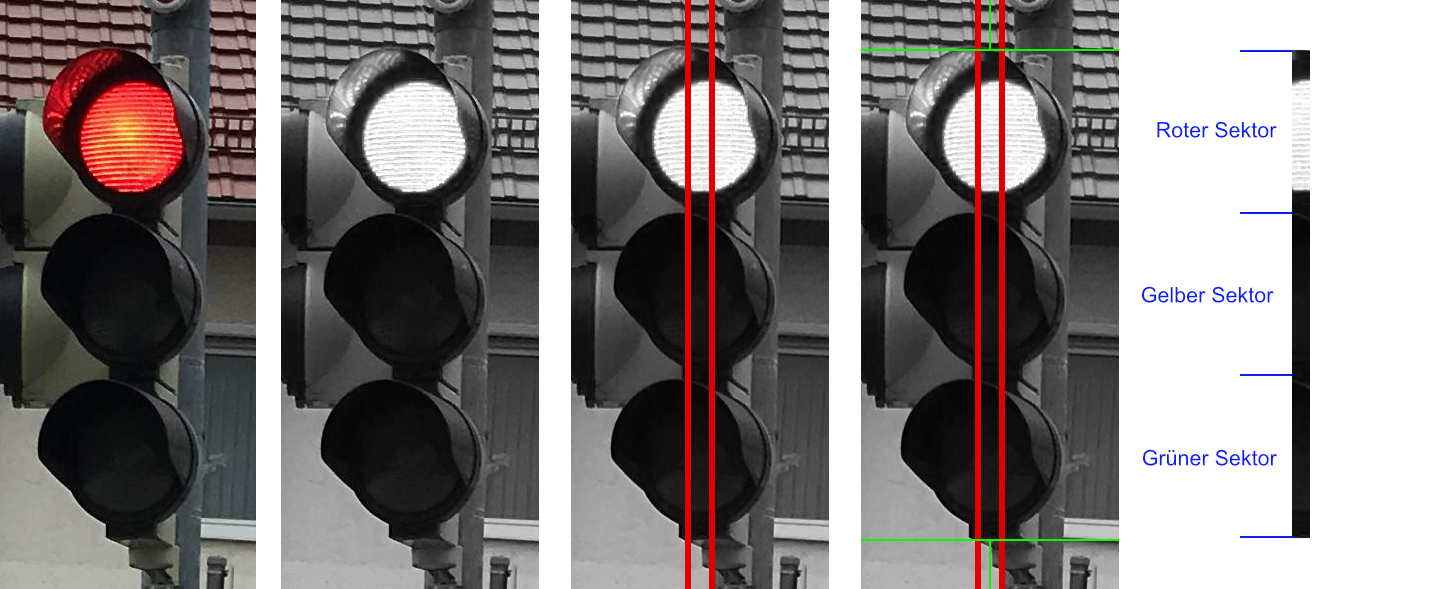
\includegraphics[width=\linewidth]{TLCropping.jpg}
			\caption{Analyse schritte}
			\label{fig:TLCrop}
		\end{figure}
		Weiterhin wurde versucht ausschließlich die einzelnen Ampelleuchten wahrzunehmen. Dadurch sollte eine genaue Phasenerkennung stattfinden. Diese Detektion wird im Folgekapitel beschrieben.
		\section{Kreiserkennung (PM)}
		Im nächsten Ansatz sollten die einzelnen Rundungen der Ampel durch Kantenerkennung erfasst werden. Ziel dieses Verfahrens ist es, die einzelnen Ampellichter herauszufiltern, um danach herausfinden zu können welche der Leuchten eingeschaltet ist. Dafür wurde OpenCV als mögliche Lösung gewählt, da diese Bibliothek bereits eine Funktion beinhaltet, die in der Lage ist, Kreise zu detektieren und zu zeichnen. In den folgenden Code Zeilen (Kreiserkennung Code~\ref{lst:KreisCode}) wird versucht, die Kreise in einem vorgegebenen Bild zu erkennen.
		\lstinputlisting[language=Python, firstline=14,lastline=17,basicstyle=\tiny,caption={Kreiserkennung Code},captionpos=b,label={lst:KreisCode}]{Kreiserkennung.py}
		Dabei legt param1 den Threshold der Kantenerkennung und param2 den Akkumulator Threshold des Kreiszentrums fest. Hier geeignete Werte universell für jedes Bild herauszufinden ist eine große Herausforderung und nahezu nicht möglich. Es gibt Bilder, in welchen diese Erkennung erstaunlich gut funktioniert, allerdings ist dieses Verfahren insgesamt zu ungenau. Auch bei Bildern mit klar erkennbaren Kreiskanten sind die gezeichneten Kreise nicht genau genug positioniert.
		\begin{figure}[h!]
			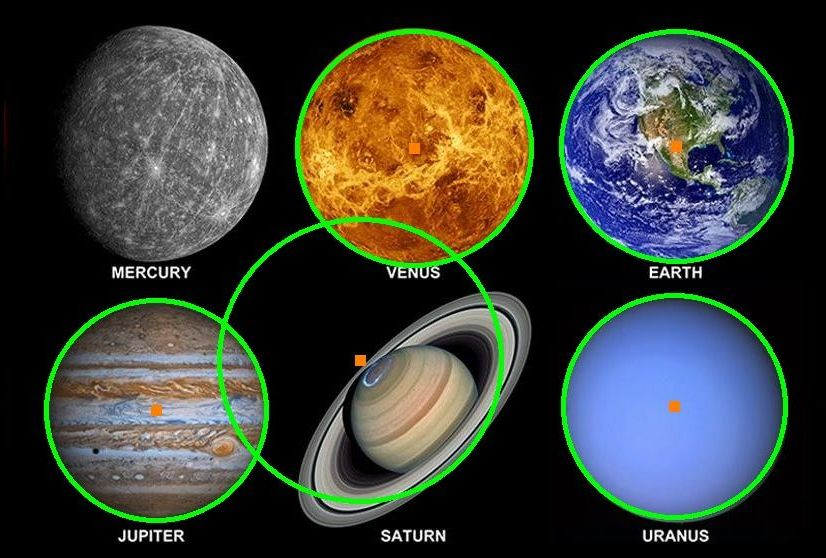
\includegraphics[width=\linewidth]{circles_detected.jpg}
			\caption{Beispielbild erkannte Kreise}
			\label{fig:CirclesDetected}
		\end{figure}
		\newline
		Folglich wurde sich gegen die OpenCV Kreiserkennung entschieden, da die Wahrscheinlichkeit zu gering ist, um die einzelnen Ampelrundungen zu erkennen.
		\section{Umsetzung (MM)}
		Für das Image Processing und die Image Analyse wurde die Scriptsprache Python verwendet um ein einfaches prototypisches implementieren der Algorithmen zu ermöglichen. Bei erfolgreichen Prototyp wäre das Programm in C portiert worden um die Berechnungszeit zu verringern. Es wurden zunächst Testbilder verwendet, welche mit der Python Bibliothek openCV eingelesen und zugeschnitten wurden. Außerdem wurde numpy verwendet um den Umgang mit den Bildarrays zu erleichtern (vgl. Code~\ref{lst:ImgCropCode} und Code~\ref{lst:ImgAnalyCode}). Um die Bilder von darknet in Python zu nutzen wird der Wrapper darknetpy\footnote{https://github.com/danielgatis/darknetpy, besucht am 31.05.2020} verwendet.
		\lstinputlisting[language=Python, firstline=8,lastline=61,basicstyle=\tiny,caption={Auszug aus dem Image cropping Code},captionpos=b,label={lst:ImgCropCode}]{ImageProcessingPrototype.py}
		\lstinputlisting[language=Python, firstline=77,lastline=118,basicstyle=\tiny,caption={Auszug aus dem Image Analyse (greyscale) Code},captionpos=b,label={lst:ImgAnalyCode}]{ImageProcessingPrototype.py}
		\section{Probleme dieses Ansatzes (MM)}
		Insgesamt bringt dieser Ansatz mangelhafte Ergebnisse. Viele Detektionen sind falsch oder knapp richtig (Unterschiede in den Sektoren sind gering). Das Zuschneiden in x-Richtung muss sich auf eine möglichst richtige Bbox verlassen, da sich die Ampel ansonsten nicht mittig des Ausschnitts befindet. Die Genauigkeit des Zuschneiden in y-Richtung ist stark abhängig von den Licht und Umgebungsverhältnissen und somit nicht verlässlich einsetzbar. Weitere Probleme bei der Detektion der Grenzen entstehen, wenn die Ampel nicht Schwarz ist, was in einigen Ländern, wie zum Beispiel in Großbritannien, häufig vorkommen kann. Hinzu kommt, dass dieses System nur funktional ist, wenn die Ampel aufrecht hängt. Da nur eines dieser Probleme auftreten muss um das Ergebnis zu verfälschen, wurde der Versuch die Ampelphasen durch Image Processing zu erkennen im finalen Ergebnis nicht eingesetzt und es wurde eine Lösung mit einem neuronalen Netz realisiert. \newline Im letzten Kapitel werden die Erkenntnisse dieser Studienarbeit resümiert.
		
		
	\end{onehalfspace}
	
	\chapter{Schlusswort}
	\begin{onehalfspace}
		Als Ergebnis präsentiert die Studienarbeit eine funktionstüchtige Tiny-YOLO künstliche Intelligenz, die in der Lage ist, Ampelphasen und Straßenschilder zu erkennen. Dabei werden die Straßenschilder nur erkannt, damit der Algorithmus nicht fälschlicherweise ein Schild als Ampel erkennen kann, da dies, speziell bei Parkverbotsschilder, ein großes Problem darstellte. In seltenen Fällen kann dieses dennoch eintreten. Insgesamt läuft das System mit Tiny-YOLO sehr gut und performant (ca. 58 fps) auf einem Laptop (CUDA + CUDNN + OPENCV (GTX1050)). In Zukunft kann dieses Projekt auf den NVIDIA Jetson ausgeweitet werden, damit eine "`mobile"' Version der Detektion entstehen kann. Da die Technische Hochschule Deggendorf zu Corona-Zeiten keinen Jetson Nano mehr für diese Studienarbeit zur Verfügung stellen konnte, konnte das Projekt nur auf herkömmlichen PC-Systemen bearbeitet werden. Es stand kurzzeitig ein privater NVIDIA Jetson Nano zur Verfügung, um die Performanz der künstlichen Intelligenz unter Probe zu stellen. Dabei war es möglich mit dem Jetson eine Bilderkennung von bis zu 21 Bildern pro Sekunde zu erreichen (siehe Abbildung~\ref{fig:Jetson}).
		\begin{figure}[h!]
			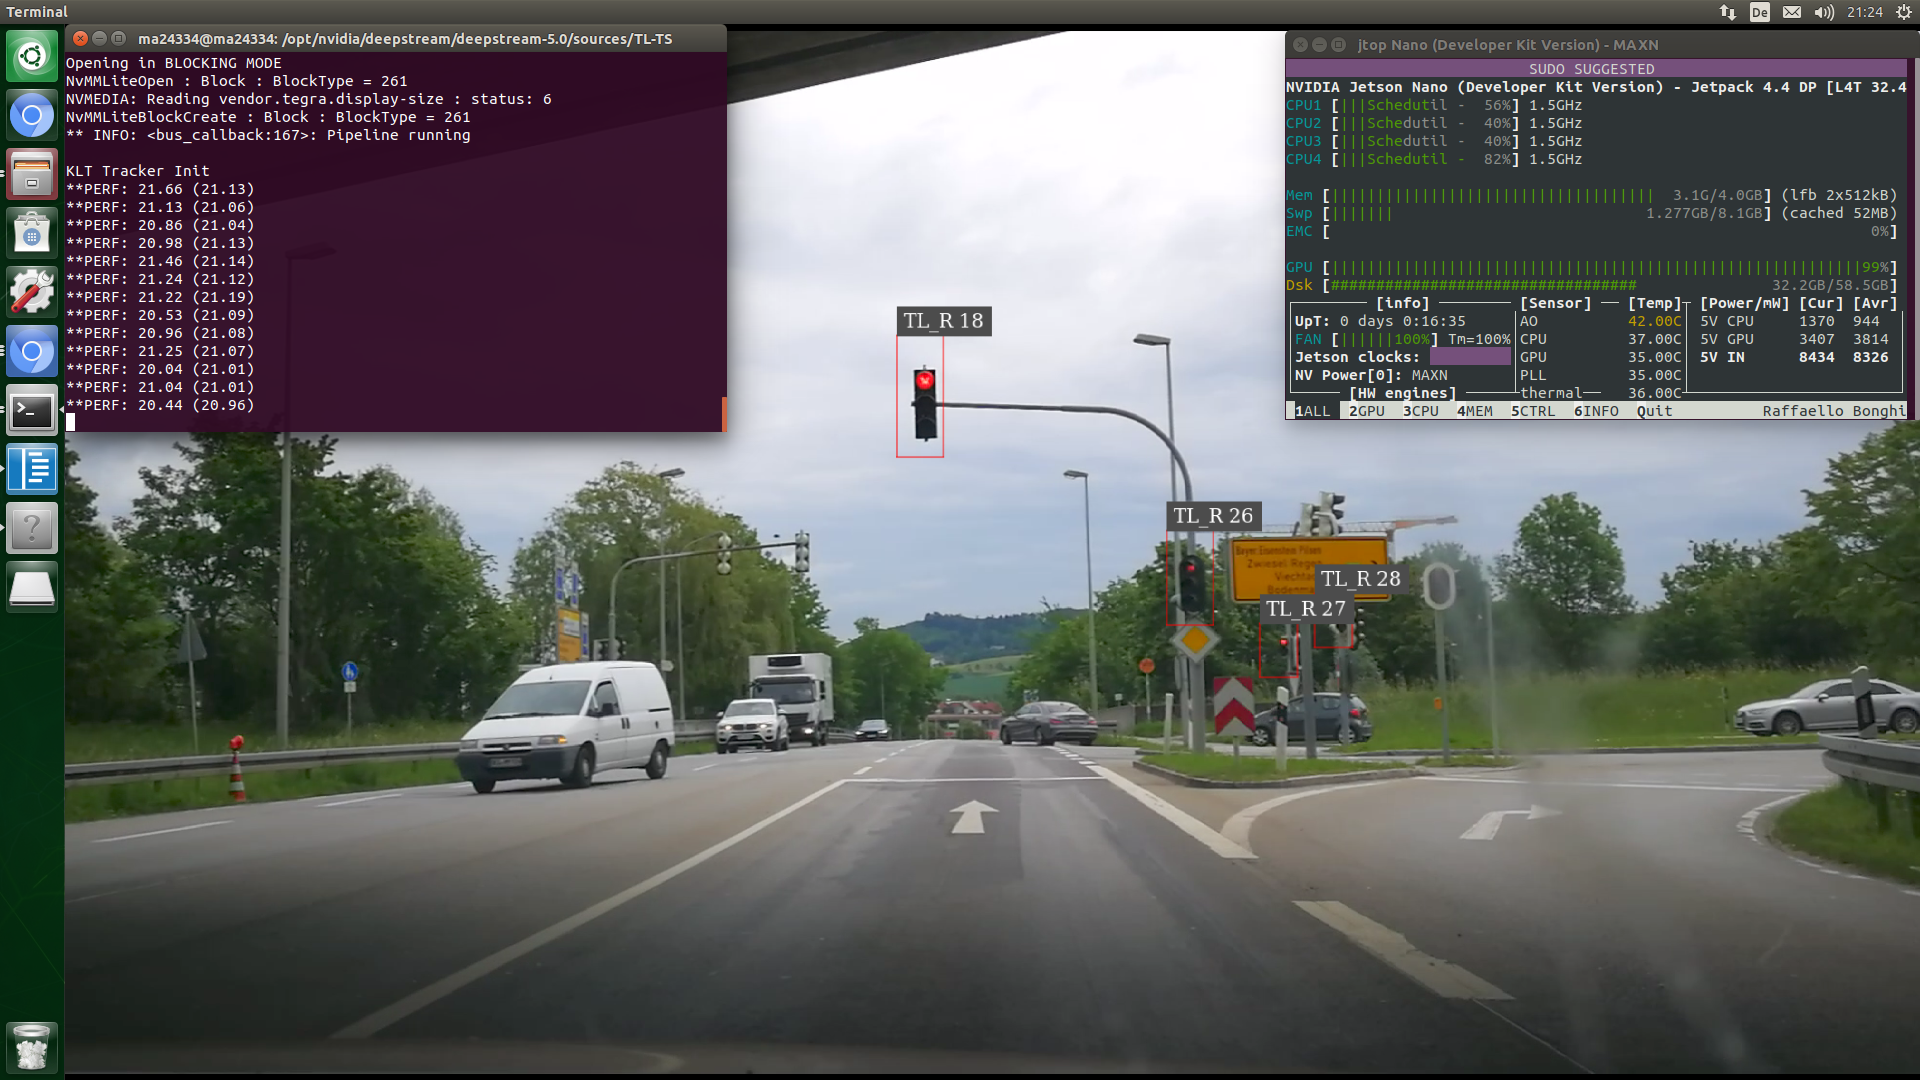
\includegraphics[width=\linewidth]{Jetson.png}
			\caption{Jetson Momentaufnahme}
			\label{fig:Jetson}
		\end{figure}
		Da der Jetson nach einem Tag wieder zurückgegeben werden musste, konnten keine weiteren Tests und Optimierungen auf dieser Platform ausgeführt werden. Die Werte sind in jedem Fall gut genug, dass eine mobile Variante mit diesem umsetzbar wäre. Damit die weitere Bilderkennung präziser gestaltet werden kann, sollten schnelle geeignete "`Image Processing"'-Verfahren genutzt werden. Diese wurden jedoch nicht angewandt, da sie zu ungenau beziehungsweise zu laufzeitaufwendig waren.
	\end{onehalfspace}
	
\end{document}
